% ──────────────────────────────────────────────
% BÁO CÁO DỰ ÁN CH2021 - ĐỔI MỚI SÁNG TẠO & KHỞI NGHIỆP
% Đề tài: Nền tảng trợ lý ảo chấm điểm và chỉnh sửa form
%         tập Calisthenics thời gian thực
% ──────────────────────────────────────────────
\documentclass[a4paper,12pt]{article}

% ─── Font & Encoding ───
\usepackage[T5]{fontenc}
\usepackage[utf8]{inputenc}
\usepackage[vietnamese]{babel}
\usepackage{times}

% ─── Geometry ───
\usepackage[top=2cm, bottom=2cm, left=3cm, right=2cm]{geometry}

% ─── Packages ───
\usepackage{graphicx}
\usepackage{tikz}
\usepackage{amsmath,amssymb}
\usepackage{booktabs}
\usepackage{array}
\usepackage{enumitem}
\usepackage{hyperref}
\usepackage{fancyhdr}
\usepackage{caption}
\usepackage{float}
\usepackage{listings}
\usepackage{xcolor}
\usepackage{multirow}

% ─── Hyperlinks ───
\hypersetup{
    colorlinks=true,
    linkcolor=black,
    urlcolor=blue,
    citecolor=black,
}

% ─── Header/Footer ───
\pagestyle{fancy}
\fancyhf{}
\fancyhead[L]{CH2021 -- Đổi mới sáng tạo và Khởi nghiệp}
\fancyhead[R]{Fitness AI Coach}
\fancyfoot[C]{\thepage}
\renewcommand{\headrulewidth}{0.4pt}

% ─── Paragraph formatting ───
\setlength{\parindent}{0.5cm}
\setlength{\parskip}{6pt}

% ─── Code listing style ───
\lstdefinestyle{pythonstyle}{
    language=Python,
    basicstyle=\ttfamily\footnotesize,
    keywordstyle=\color{blue},
    commentstyle=\color{gray},
    stringstyle=\color{red},
    numbers=left,
    numberstyle=\tiny\color{gray},
    frame=single,
    breaklines=true,
}

% ─── Begin document ───
\begin{document}

% ─── Title Page ───
\begin{titlepage}
    \begin{tikzpicture}[remember picture, overlay]
        \draw[line width=0.4pt] ([xshift=3cm,yshift=2cm]current page.south west) rectangle ([xshift=-2cm,yshift=-2cm]current page.north east);
        \draw[line width=0.4pt] ([xshift=3.15cm,yshift=2.15cm]current page.south west) rectangle ([xshift=-2.15cm,yshift=-2.15cm]current page.north east);
    \end{tikzpicture}
    \centering
    \vspace*{1.5cm}

    {\LARGE ĐẠI HỌC BÁCH KHOA HÀ NỘI}\\[4pt]
    {\large HỌC PHẦN CH2021}\\[4pt]
    {\large ĐỔI MỚI SÁNG TẠO VÀ KHỞI NGHIỆP}\\[20pt]

    
\includegraphics[width=5cm]{document/logo.png}\\[25pt]

    {\huge\bfseries BÁO CÁO DỰ ÁN}\\[10pt]
    {\Large\itshape Nền tảng trợ lý ảo chấm điểm và chỉnh sửa\\[4pt]
    form tập Calisthenics thời gian thực}\\[4pt]
    {\large (Fitness AI Coach)}\\[30pt]

    \begin{tabular}{rl}
        \textbf{Nhóm:} & Nothing is Impossible \\[6pt]
        \textbf{Thành viên:} & Phạm Hải Duy -- 202400102 \\
        & Nguyễn Minh Dũng -- 202416682 \\
        & Trần Duy Anh -- 20234737 \\
        & Phạm Xuân Sơn -- 202416065 \\
        & Trần Quang Hùng -- 20235941 \\
        & Phạm Hồng Hải -- 202417851 \\
        & Nguyễn Tuấn Nam -- 20231029 \\[20pt]
        \textbf{Giảng viên hướng dẫn:} & Nguyễn Thị Minh Phương \\[6pt]
    \end{tabular}\\[40pt]

    {\large HÀ NỘI, 06/2025}
\end{titlepage}

% ─── Table of Contents ───
\newpage
\tableofcontents
\newpage

% ══════════════════════════════════════════════
% 1. MÔ TẢ THỰC TRẠNG / VẤN ĐỀ
% ══════════════════════════════════════════════
\section{Mô tả thực trạng / Vấn đề}

\subsection{Nhu cầu lớn đối nghịch rào cản tài chính}
Qua số liệu khảo sát thực tế, giới trẻ có nhu cầu cải thiện vóc dáng và sức khỏe cực kỳ cao. Tuy nhiên, mức chi phí thuê Huấn luyện viên cá nhân (PT) truyền thống dao động từ 300.000đ -- 800.000đ/buổi, vượt xa khả năng chi trả của học sinh, sinh viên.

\subsection{Hệ lụy chấn thương từ việc tự tập sai tư thế}
Xu hướng tự học Calisthenics qua các video ngắn trên TikTok/YouTube bùng nổ nhưng người tập không thể tự quan sát và ý thức được lỗi sai form của mình. Điều này dẫn đến tỷ lệ chấn thương nghiêm trọng ở các vùng khớp vai, cổ tay và cột sống.

\subsection{Sự lên ngôi của xu hướng tự tập luyện}
Nhóm đối tượng \lq\lq ví mỏng\rq\rq\ có xu hướng chuyển dịch mạnh mẽ sang việc tự tập tại nhà, công viên hoặc các cụm xà công cộng. Nhu cầu của họ không chỉ dừng lại ở việc tìm kiếm bài tập, mà là cần một công cụ đồng hành có thể kiểm soát chất lượng động tác để thay thế PT.

\subsection{Diện mạo đối thủ cạnh tranh và nỗi đau thị trường}
Hiện tại, người tập thường tìm đến hai nhóm giải pháp thay thế, nhưng cả hai đều để lại những \lq\lq nỗi đau\rq\rq\ cực kỳ lớn:

\textbf{Nỗi đau từ nhóm đối thủ \lq\lq Ứng dụng lịch trình/Giáo án Gym tĩnh\rq\rq:} Các ứng dụng phổ biến hiện nay (Hevy, Strong, ứng dụng theo dõi lịch tập) chỉ đóng vai trò như một cuốn sổ tay ghi chép thuần túy. Chúng cung cấp danh sách bài tập, số lượng reps/sets mẫu và đếm thời gian nghỉ, nhưng hoàn toàn \lq\lq mù\rq\rq\ trước chuyển động thực tế của người dùng. Hệ thống không thể phát hiện người tập có đang gù hông khi squat, hay ăn gian biên độ (half-rep) khi hít đất. Người dùng có cảm giác an tâm ảo là mình đang theo sát lộ trình, nhưng thực tế việc tập sai form tích lũy theo ngày tháng chính là nguyên nhân hàng đầu dẫn đến chấn thương.

\subsection{Lỗ hổng công nghệ đối sánh cũ}
Các giải pháp AI nhận diện tư thế hiện tại thường áp dụng đối sánh khoảng cách pixel tuyệt đối. Khi so sánh một người mẫu cao 1m80 với một sinh viên cao 1m65, hệ thống sẽ báo lỗi sai lệch hoàn toàn do sự khác biệt về chiều cao và tỷ lệ các phân đoạn khung xương. Đây là bài toán \textbf{bất biến tỷ lệ cơ thể} (scale-invariant pose matching) mà dự án giải quyết triệt để.

\subsection{Dữ liệu khảo sát chứng minh nhu cầu thị trường}
Dự án đã tiến hành khảo sát thực tế với 43 mẫu phản hồi, ghi nhận các chỉ số quan trọng trong Bảng \ref{tab:survey}.

\begin{table}[H]
    \centering
    \caption{Kết quả khảo sát nhu cầu thị trường}
    \label{tab:survey}
    \begin{tabular}{p{7cm}p{2.5cm}p{5cm}}
        \toprule
        \textbf{Chỉ số khảo sát} & \textbf{Tỷ lệ} & \textbf{Ý nghĩa} \\
        \midrule
        Độ tuổi trọng tâm 18--21 & 74.4\% & Xác thực phân khúc Gen Z \\
        Nhu cầu tập Gym \& Calisthenics & 72.1\% & Dung lượng thị trường ngách đủ lớn \\
        Đánh giá động tác khó, nhiều kỹ thuật & 65.1\% & Rất cần PT giám sát \\
        Sẵn sàng trải nghiệm Web chỉnh form & 83.8\% & Mức độ đón nhận sản phẩm cao \\
        Ngân sách chi trả 0--40.000đ & 53.5\% & Phù hợp gói thuê bao 15--30k/tháng \\
        \bottomrule
    \end{tabular}
\end{table}

% ══════════════════════════════════════════════
% 2. NỘI DUNG Ý TƯỞNG
% ══════════════════════════════════════════════
\section{Nội dung ý tưởng}

\subsection{Tổng quan giải pháp}
\textbf{Fitness AI Coach} là nền tảng Web App tinh gọn (PWA) sử dụng thị giác máy tính và trí tuệ nhân tạo để phân tích tư thế tập luyện Calisthenics theo thời gian thực. Hệ thống so sánh khung xương người tập với khung xương mẫu chuẩn, đưa ra điểm số và phản hồi lỗi tức thì. Mã nguồn dự án được công khai tại \url{https://github.com/haiduy1711/MovementChecker}.

\subsection{Công nghệ cốt lõi}

\subsubsection{Chuẩn hóa tư thế bất biến tỷ lệ (Scale-invariant Pose Matching)}
Hệ thống trích xuất 33 điểm khớp xương theo chuẩn MediaPipe / Human3.6M, sau đó chuẩn hóa bằng hai bước:

\begin{enumerate}[leftmargin=*,label=\textbf{Bước \arabic*.}]
    \item \textbf{Tịnh tiến khớp gốc:} Trừ tọa độ khớp chậu (Root/Pelvis, chỉ số 0) về gốc tọa độ $(0,0)$.
    \item \textbf{Chuẩn hóa tỷ lệ:} Chia toàn bộ tọa độ cho độ dài cột sống $\|\text{joint}[8]-\text{joint}[0]\|$.
\end{enumerate}

Sau chuẩn hóa, 12 vector xương được so sánh bằng độ tương đồng cosine (cosine similarity):

\begin{equation}
    \text{cos\_sim}(\mathbf{a}, \mathbf{b}) = \frac{\mathbf{a} \cdot \mathbf{b}}{\|\mathbf{a}\| \,\|\mathbf{b}\|}
    \label{eq:cosine}
\end{equation}

Hai vector cùng hướng cho cosine gần bằng 1, bất kể độ dài khác nhau (Hình \ref{fig:cosine}). Khoảng cách hiệu chỉnh (move\_distance) được tái cấu trúc động theo tỷ lệ nhân trắc học riêng biệt của từng cá nhân, loại bỏ lỗi lệch chiều cao.

\begin{figure}[H]
    \centering
    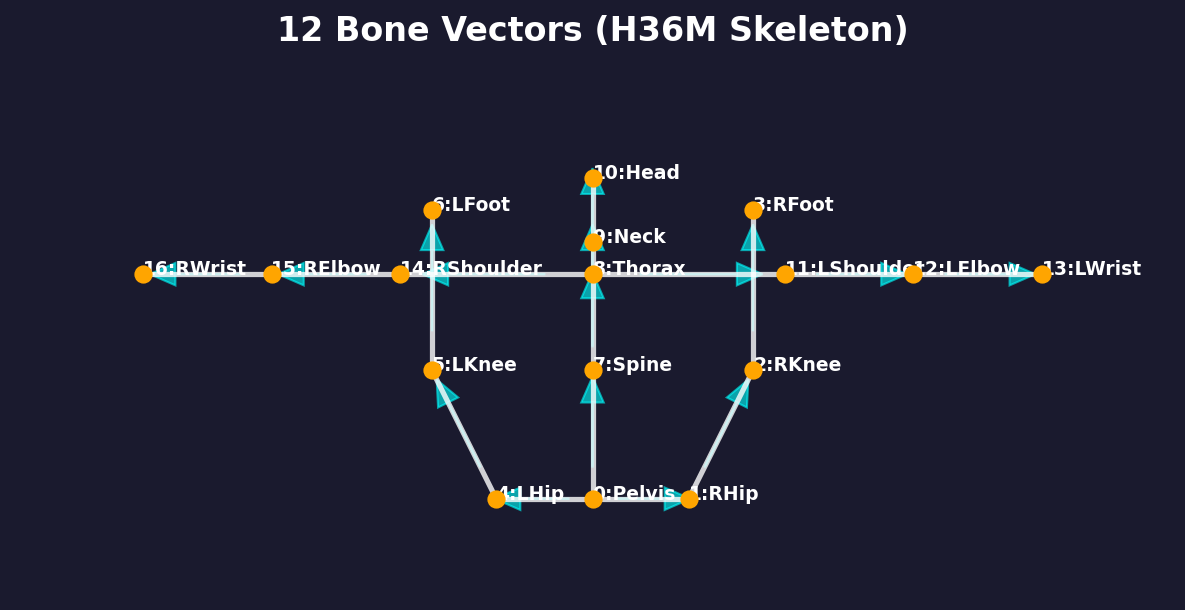
\includegraphics[width=0.6\textwidth]{document/h36m_12_bone_vectors.png}
    \caption{Minh họa 12 vector xương H36M được so sánh}
    \label{fig:cosine}
\end{figure}

\subsubsection{Pipeline xử lý dữ liệu tinh gọn}
Pipeline được thiết kế hai chế độ (Hình \ref{fig:pipeline}):

\begin{itemize}
    \item \textbf{Offline (Calibration):} Sử dụng YOLO Pose một lần duy nhất để xử lý video mẫu, chuyển đổi COCO 17 $\rightarrow$ H36M 17, trích xuất 30 keyframes bằng thuật toán K-Means, chuẩn hóa vector và đóng gói thành tệp NPZ/PKL (dung lượng $<10$ KB).
    \item \textbf{Real-time (Inference):} Sử dụng MediaPipe Pose (tốc độ 52+ FPS trên CPU) để nhận diện khung xương trực tiếp từ webcam. Bộ lọc trung bình động (rolling window = 7 frames) làm mượt nhiễu.
\end{itemize}

\begin{figure}[H]
    \centering
    \begin{minipage}{0.9\textwidth}
    \begin{verbatim}
    Video mẫu (MP4)
         |
    [YOLO / MediaPipe Pose]
         |
    COCO 17 / MediaPipe 33 landmarks
         |
    [coco_to_h36m / mediapipe_to_h36m]
         |
    H36M 17 joints (x, y, confidence)
         |
    [K-Means n_clusters=30]
         |
    30 Keyframes
         |
    [normalize_pose: centering + scaling]
         |
    NPZ / PKL Checkpoints (raw + norm)
    \end{verbatim}
    \end{minipage}
    \caption{Pipeline xử lý dữ liệu}
    \label{fig:pipeline}
\end{figure}

\subsubsection{Hệ thống phản hồi đa phương thức thời gian thực}
\begin{itemize}
    \item \textbf{Trực quan:} Khung xương người tập được vẽ trực tiếp lên hình ảnh camera, màu \textcolor{green}{xanh} nếu đúng form, màu \textcolor{red}{đỏ} nếu sai. Mỗi xương có đầu mũi tên chỉ hướng.
    \item \textbf{Điểm số:} Công thức tính điểm:
    \begin{equation}
        \text{score} = \underbrace{\max(0,\,100 - N_{\text{err}} \times 8.33)}_{\text{bone score } \times 0.7} + \underbrace{\max(0,\,100 - N_{\text{align}} \times 10 - N_{\text{warn}} \times 5)}_{\text{align score } \times 0.3}
    \end{equation}
    \item \textbf{Âm thanh:} Text-to-Speech (Web Speech API) đọc phản hồi bằng tiếng Việt, ví dụ: \lq\lq Lưng võng, hạ hông xuống 5cm\rq\rq.
    \item \textbf{Guide skeleton:} Khung xương ảo mờ (màu vàng) hướng dẫn người dùng căn chỉnh camera trước khi bắt đầu.
\end{itemize}

\subsubsection{Quy trình đánh giá}
Hệ thống hoạt động như máy trạng thái hữu hạn (Finite State Machine):

\begin{enumerate}[leftmargin=*]
    \item \textbf{Align:} So sánh pose người tập với checkpoint đầu tiên dùng cosine similarity ngưỡng 0.3. Cần 5 frame liên tiếp đạt alignment để chuyển sang bước tiếp.
    \item \textbf{Init:} Quét toàn bộ 30 checkpoints, chọn checkpoint khớp nhất làm điểm bắt đầu.
    \item \textbf{Evaluate:} Với mỗi frame, so sánh 12 vector xương với checkpoint hiện tại. Nếu tất cả vector đạt ngưỡng (tay: 0.995, chân: 0.990, thân: 0.985, cổ: 0.3) $\rightarrow$ chuyển checkpoint tiếp theo.
    \item \textbf{Rep complete:} Khi vượt qua checkpoint cuối cùng, tăng biến đếm rep và quay lại checkpoint đầu.
\end{enumerate}

\subsection{Kiến trúc hệ thống}

\begin{figure}[H]
    \centering
    \begin{minipage}{0.85\textwidth}
    \begin{verbatim}
    cali-ai-coach/
    +-- calibrate.py          # Calibration YOLO -> NPZ
    +-- live_mediapipe.py     # Camera real-time
    +-- eval_video_mediapipe.py# Video -> MP4
    +-- output_video.py       # Video -> MP4 (YOLO)
    +-- core/
    |   +-- coco_to_h36m.py   # COCO 17 -> H36M 17
    |   +-- mediapipe_to_h36m.py # MediaPipe 33 -> H36M 17
    |   +-- keyframes.py      # K-Means keyframe extraction
    |   +-- math-helpers.js    # cosineSimilarity, scorePose
    |   +-- pose-geometry.js   # BONE_STRUCTURES, H36M_SKELETON
    |   +-- live-filter.js    # RollingPoseFilter
    |   +-- live-pipeline-v2.js # LivePoseEvaluator (FSM)
    |   +-- adapter.js        # normalizePose, mediapipe33toH36M
    +-- web/
    |   +-- app.py            # Flask server
    |   +-- evaluator.py      # Evaluation logic
    |   +-- templates/        # HTML templates
    |   +-- static/           # CSS, JS, checkpoints
    +-- data/
        +-- calib_checkpoints.npz  # 30 keyframes
        +-- pose_landmarker_full.task  # MediaPipe model
    \end{verbatim}
    \end{minipage}
    \caption{Cấu trúc thư mục dự án}
    \label{fig:structure}
\end{figure}

% ══════════════════════════════════════════════
% 3. PHÂN TÍCH THỊ TRƯỜNG
% ══════════════════════════════════════════════
\section{Phân tích thị trường}

Cơ sở định giá để tính toán quy mô thị trường dựa trên mức phí thuê bao Premium lý tưởng: \textbf{20.000đ/tháng} (tương đương 240.000đ/năm), được xác thực qua 53.5\% số liệu khảo sát sinh viên sẵn sàng chi trả từ 0đ -- 40.000đ/tháng.

\subsection{TAM -- Total Addressable Market}
Toàn bộ thị trường người tiêu dùng tham gia tập luyện Fitness, Gym và Calisthenics số hóa tại Việt Nam. Theo thống kê ngành Fitness, Việt Nam có khoảng 15 triệu người thuộc thế hệ Gen Z và người trẻ (16--30 tuổi) có hành vi sử dụng thiết bị thông minh và quan tâm đến sức khỏe.

\begin{equation}
    \text{TAM} = 15.000.000 \times 240.000 = 3.600.000.000.000 \text{ đ/năm}
\end{equation}

\subsection{SAM -- Serviceable Available Market}
Phân khúc học sinh, sinh viên (18--25 tuổi) tại Việt Nam có nhu cầu tự tập luyện Calisthenics/Home Workout nhưng ngân sách hạn chế. Tổng số lượng sinh viên Đại học, Cao đẳng trên toàn quốc khoảng 2,2 triệu. Theo khảo sát: 72.1\% có nhu cầu tập Gym \& Calisthenics, 83.8\% sẵn sàng trải nghiệm nền tảng Web chỉnh form.

\begin{equation}
    \text{Số lượng mục tiêu SAM} = 2.200.000 \times 72.1\% \times 83.8\% \approx 1.330.000 \text{ sinh viên}
\end{equation}

\begin{equation}
    \text{SAM} = 1.330.000 \times 240.000 = 319.200.000.000 \text{ đ/năm}
\end{equation}

\subsection{SOM -- Serviceable Obtainable Market}
Sinh viên tại các cụm trường Đại học lớn khu vực Hà Nội (Đại học Bách Khoa, Đại học Kinh tế Quốc dân, Đại học Xây dựng, ...), ước tính khoảng 100.000 sinh viên. Dự án đặt mục tiêu chuyển đổi 10\% lượng sinh viên tiềm năng trong 1--2 năm đầu nhờ chiến lược Marketing 0 đồng.

\begin{equation}
    \text{Số lượng mục tiêu SOM} = 100.000 \times 60.4\% \times 10\% = 6.040 \text{ người dùng trả phí}
\end{equation}

\begin{equation}
    \text{SOM} = 6.040 \times 240.000 = 1.449.600.000 \text{ đ/năm}
\end{equation}

\begin{table}[H]
    \centering
    \caption{Tổng hợp quy mô thị trường}
    \label{tab:tam-sam-som}
    \begin{tabular}{lccr}
        \toprule
        \textbf{Chỉ số} & \textbf{Số lượng} & \textbf{Đơn giá/năm} & \textbf{Doanh thu tiềm năng} \\
        \midrule
        TAM & 15.000.000 người & 240.000đ & 3.600 tỷ đồng \\
        SAM & 1.330.000 sinh viên & 240.000đ & 319,2 tỷ đồng \\
        SOM & 6.040 người dùng & 240.000đ & 1,45 tỷ đồng \\
        \bottomrule
    \end{tabular}
\end{table}

% ══════════════════════════════════════════════
% 4. MÔ HÌNH KINH DOANH
% ══════════════════════════════════════════════
\section{Mô hình kinh doanh}

\subsection{Chi phí vận hành tối giản (Zero Server Cost)}
Toàn bộ mô hình AI và thuật toán đối sánh ma trận vector được thiết kế để xử lý trực tiếp tại trình duyệt (On-device AI). Dự án không phải gánh chi phí thuê Cloud GPU để render hay tính toán video, giúp chi phí vận hành tiệm cận mức tối thiểu, mang lại biên lợi nhuận gộp cực kỳ cao.

\subsection{Chiến lược định giá Freemium}
\begin{itemize}
    \item \textbf{Miễn phí:} Mở khóa bài tập căn bản (Hít đất, Squat, Plank).
    \item \textbf{Premium:} 15.000--30.000đ/tháng, mở khóa bài tập nâng cao (Handstand, Planche, Muscle-up) và chế độ thi đấu PvP.
    \item \textbf{Dòng doanh thu bổ trợ:} Tiếp thị liên kết (Affiliate Marketing) phân phối phụ kiện tập luyện (dây kháng lực, xà đơn, đệm cổ tay) và quảng cáo lập trình (Programmatic Ads).
\end{itemize}

\subsection{Business Model Canvas (BMC)}
\begin{table}[H]
    \centering
    \caption{Chín cấu phần của BMC}
    \label{tab:bmc}
    \begin{tabular}{|p{2.8cm}|p{11.2cm}|}
        \hline
        \textbf{Cấu phần} & \textbf{Mô tả} \\
        \hline\hline
        Đối tác chính & CLB Thể thao, Ban Quản lý Ký túc xá các trường Đại học; đơn vị cung cấp dụng cụ tập luyện (đối tác Affiliate) \\
        \hline
        Hoạt động chính & Phát triển thuật toán đồ thị xương và Cosine Similarity; trích xuất keyframes bài tập mẫu (.pkl); tổ chức chiến dịch GTM tại xà đơn công cộng \\
        \hline
        Giá trị đề xuất & Trợ lý ảo chấm điểm form thời gian thực, bất biến tỷ lệ cơ thể; chi phí siêu rẻ (15k--30k/tháng); an toàn tuyệt đối cho xương khớp \\
        \hline
        Quan hệ KH & Tự phục vụ (Self-service) qua Web App; chăm sóc tự động, xây dựng cộng đồng giao lưu điểm số, vinh danh \\
        \hline
        Phân khúc KH & Sinh viên 18--21 tuổi, ngân sách hạn chế (\lq\lq ví mỏng\rq\rq), đam mê tập luyện \\
        \hline
        Nguồn lực chính & Thuật toán AI tinh gọn chạy Client; bản quyền mã nguồn PWA và tệp dữ liệu bài tập; đội ngũ kỹ thuật \\
        \hline
        Kênh truyền thông & O2O (Online to Offline): QR code tại cụm xà công cộng; truyền thông 0 đồng nhờ người dùng chia sẻ TikTok \\
        \hline
        Cơ cấu chi phí & Zero Server Cost (xử lý On-device); chi phí in ấn QR; duy trì tên miền, bảo mật, bản quyền công cụ \\
        \hline
        Dòng doanh thu & Freemium Premium (15k--30k/tháng); Affiliate Marketing phụ kiện; Programmatic Ads \\
        \hline
    \end{tabular}
\end{table}

\subsection{Trọng tài AI và hệ thống thi đấu PvP}
Ứng dụng độ chính xác của thuật toán cos\_sim để tạo ra hệ thống \lq\lq Trọng tài AI\rq\rq\ công tâm, đếm rep chuẩn, loại bỏ gian lận form. Triển khai tính năng PvP trực tuyến (thách đấu liên trường giữa các Đại học) nhằm kích thích bản sắc cộng đồng và tính ganh đua.

\subsection{Chiến lược Marketing 0 đồng (Organic Viral)}
Tích hợp tính năng tự động xuất bản video highlight buổi tập có phủ khung xương AI đổi màu và điểm số. Người dùng chia sẻ lên TikTok, Facebook Reels, Instagram Stories, tạo hiệu ứng lan tỏa tự nhiên không tốn ngân sách chuyển đổi khách hàng (CAC).

\subsection{Điểm chạm offline cộng đồng}
Triển khai dán bảng biểu chứa mã QR kích hoạt nhanh tại hệ thống cụm xà đơn, xà kép công cộng trong khuôn viên ký túc xá, công viên và sân thể thao của trường đại học mục tiêu.

% ══════════════════════════════════════════════
% 5. ĐỘI NGŨ THỰC HIỆN
% ══════════════════════════════════════════════
\section{Đội ngũ thực hiện}

\subsection{Thành viên nhóm Nothing is Impossible}
\begin{table}[H]
    \centering
    \caption{Thành viên và phân công nhiệm vụ}
    \label{tab:team}
    \begin{tabular}{p{1.8cm}p{2.5cm}p{2.8cm}p{1cm}p{5.5cm}}
        \toprule
        \textbf{MSSV} & \textbf{Họ và tên} & \textbf{Ngành học} & \textbf{Khóa} & \textbf{Vai trò / Nhiệm vụ} \\
        \midrule
        202400102 & Phạm Hải Duy & CTTT Data Science \& AI & K69 & Thuật toán đối sánh, Xử lý dữ liệu, Backend Flask, Tích hợp MediaPipe \\
        202416682 & Nguyễn Minh Dũng & CTTT Data Science \& AI & K69 & Frontend Web, Tích hợp MediaPipe, Web API \\
        20235941  & Trần Quang Hùng & CTTT Global ICT & K68 & Kiểm thử hệ thống, Phát triển tính năng \\
        20234737  & Trần Duy Anh & Nhiệt & K68 & Thiết kế UI/UX, Khảo sát người dùng \\
        202416065 & Phạm Xuân Sơn & Nhiệt & K69 & Kiểm thử sản phẩm, Đánh giá trải nghiệm \\
        202417851 & Phạm Hồng Hải & Cơ khí & K69 & Kết nối CLB thể thao, Tiếp cận người dùng đầu \\
        20231029  & Nguyễn Tuấn Nam & Kỹ thuật hóa học & K68 & Tài liệu dự án, Kiểm thử chức năng \\
        \bottomrule
    \end{tabular}
\end{table}

\subsection{Chuyên gia cần huy động}
Để hoàn thiện sản phẩm, dự án cần tham vấn chuyên gia trong các lĩnh vực:
\begin{itemize}
    \item \textbf{Huấn luyện viên Calisthenics chuyên nghiệp:} Đảm bảo độ chính xác của các tiêu chuẩn form mẫu.
    \item \textbf{Chuyên gia AI/Computer Vision:} Tối ưu hóa mô hình Pose Estimation cho thiết bị cấu hình thấp.
\end{itemize}

% ══════════════════════════════════════════════
% 6. TÀI LIỆU THAM KHẢO
% ══════════════════════════════════════════════
\section{Tài liệu tham khảo}

\begin{enumerate}[label={[\arabic*]}]
    \item Bazarevsky, V., et al. (2020). \textit{BlazePose: On-device Real-time Body Pose Tracking}. Google Research. -- Cơ sở kiến trúc mạng thần kinh tích chập siêu nhẹ, nền tảng tối ưu hóa mô hình PWA chạy On-device.

    \item Lugaresi, C., et al. (2019). \textit{MediaPipe: A Framework for Building Perception Pipelines}. Google Research. -- Tài liệu kỹ thuật nền tảng chứng minh tính ổn định và tốc độ xử lý luồng dữ liệu khung xương 33 điểm.

    \item Ionescu, C., et al. (2014). \textit{Human3.6M: Large Scale Datasets and Predictive Methods for 3D Human Sensing in Natural Environments}. IEEE TPAMI. -- Tập dữ liệu chuẩn cho cấu trúc khớp xương người, củng cố giải pháp xử lý tọa độ không gian 3D.

    \item Zhu, Y., et al. (2018). \textit{Learning to Estimate 3D Human Pose from a Single Image using Cosine Similarity}. IEEE CVPR. -- Minh chứng học thuật bảo vệ phương pháp sử dụng góc khớp hình học và vector khoảng cách tương đối, xử lý triệt để bài toán bất biến tỷ lệ cơ thể.

    \item Lea, C., et al. (2017). \textit{Temporal Convolutional Networks for Action Segmentation and Detection}. IEEE CVPR. -- Lý thuyết nền tảng phân đoạn chuỗi hành động theo thời gian, hỗ trợ logic sliding window và FSM nhận diện pha chuyển động.

    \item Vemulapalli, R., et al. (2014). \textit{Human Action Recognition by Representing 3D Skeletons as Points in a Lie Group}. IEEE CVPR. -- Cơ sở toán học ánh xạ khung xương thành điểm trong không gian nhóm Lie, tối ưu hệ thống Trọng tài AI đếm lượt tập.
\end{enumerate}

\end{document}
